Este reporte reúne lo que el simulador dice del Xitle II, el
cohete híbrido de Propulsión UNAM que voló en Spaceport
America el 22 de junio de 2024. Cada sección da los números,
explica de dónde salen físicamente y dice qué implican para
el diseño. Al final comparo con el vuelo real.

Todos los valores salen del código de este repositorio con
la configuración por defecto
(\texttt{Simulador/src/XitleFile.py} y
\texttt{Simulador/GUI/backend.py}), el sitio y la atmósfera
del día del vuelo, vuelo libre e integrador DOP853, con la
semilla de viento 2024. La última sección explica cómo
repetirlos.

\section{Resumen}\label{resumen}

{\def\LTcaptype{none} % do not increment counter
\begin{longtable}[]{@{}
  >{\raggedright\arraybackslash}p{(\linewidth - 2\tabcolsep) * \real{0.5000}}
  >{\raggedright\arraybackslash}p{(\linewidth - 2\tabcolsep) * \real{0.5000}}@{}}
\toprule\noalign{}
\begin{minipage}[b]{\linewidth}\raggedright
Cantidad
\end{minipage} & \begin{minipage}[b]{\linewidth}\raggedright
Valor
\end{minipage} \\
\midrule\noalign{}
\endhead
\bottomrule\noalign{}
\endlastfoot
Longitud y diámetro & 4.266 m y 0.152 m \\
Masa al despegue y sin propelente & 46.6 kg y 31.5 kg \\
Impulso total del motor & 21 139 N·s \\
Margen estático al despegue y al fin del quemado & 2.75 y
4.22 calibres \\
Velocidad al salir del riel & 25.3 m/s \\
Aceleración máxima & 44.9 m/s² (4.6 g) \\
Velocidad máxima & 343 m/s (Mach 1.01) \\
Apogeo sobre el sitio & 7083 m a los 41.7 s \\
Apogeo medido en el vuelo real & 6573 m \\
\end{longtable}
}

Lo que más pesa del análisis:

\begin{enumerate}
\def\labelenumi{\arabic{enumi}.}
\tightlist
\item
  \textbf{El cohete es estable en todo el vuelo}, con margen
  de sobra. El margen crece de 2.75 a 4.22 calibres conforme
  se vacían los tanques.
\item
  \textbf{El motor entrega casi todo su impulso en la
  primera mitad del quemado.} A los 10.4 s ya dio el 90 \%.
  Los 11 s restantes empujan menos que el arrastre.
\item
  \textbf{El cohete llega justo a Mach 1}, que es donde el
  arrastre es mayor y donde las fórmulas de estabilidad
  dejan de ser confiables.
\item
  \textbf{El fuselaje está muy lejos de su límite
  estructural}, con márgenes de +80 o más. Las aletas no:
  con las propiedades de catálogo, el cohete vuela nueve
  segundos por encima de su velocidad de flameo.
\item
  \textbf{El paracaídas principal es chico para la masa del
  cohete.} Con las dos etapas el cohete aterriza a 12.3 m/s.
\item
  \textbf{El simulador da un apogeo 7.8 \% mayor que el
  medido.} La diferencia se acumula toda entre los 5 y los
  15 s de vuelo, durante el quemado. Después de los 20 s la
  velocidad simulada y la medida coinciden.
\end{enumerate}

\section{El cohete}\label{el-cohete}

El Xitle II tiene 4.266 m de largo y 0.152 m de diámetro,
una relación de 28 a 1. Es un cohete muy esbelto.

\begin{figure}
\centering
\pandocbounded{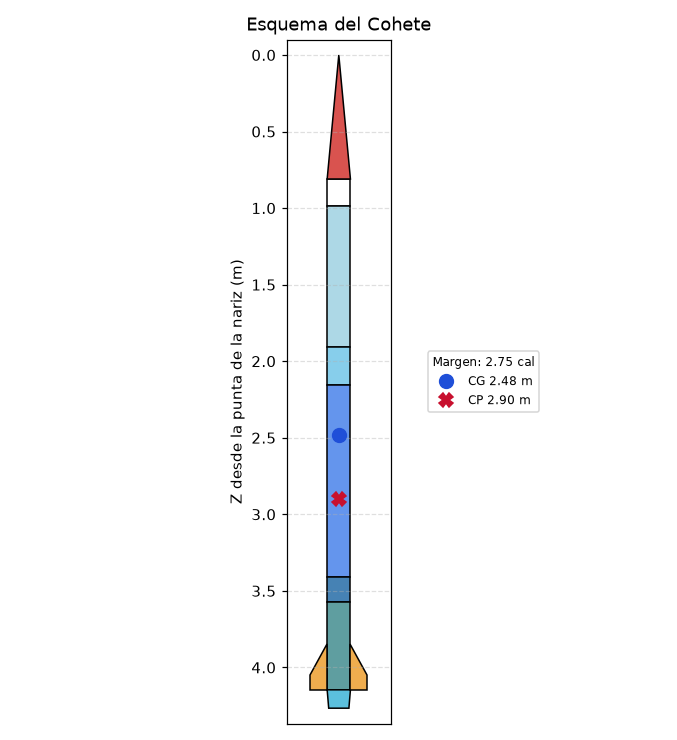
\includegraphics[keepaspectratio,alt={Esquema
del Xitle II con su centro de gravedad y su centro de
presión}]{figuras/esquema-cohete.png}}
\caption{Esquema del Xitle II con su centro de gravedad y su
centro de presión}
\end{figure}

{\def\LTcaptype{none} % do not increment counter
\begin{longtable}[]{@{}
  >{\raggedright\arraybackslash}p{(\linewidth - 4\tabcolsep) * \real{0.3333}}
  >{\raggedright\arraybackslash}p{(\linewidth - 4\tabcolsep) * \real{0.3333}}
  >{\raggedright\arraybackslash}p{(\linewidth - 4\tabcolsep) * \real{0.3333}}@{}}
\toprule\noalign{}
\begin{minipage}[b]{\linewidth}\raggedright
Componente
\end{minipage} & \begin{minipage}[b]{\linewidth}\raggedright
Masa (kg)
\end{minipage} & \begin{minipage}[b]{\linewidth}\raggedright
Centro de gravedad (m desde la punta)
\end{minipage} \\
\midrule\noalign{}
\endhead
\bottomrule\noalign{}
\endlastfoot
Nariz (ojiva, 0.81 m) & 0.80 & 0.61 \\
Aviónica & 1.80 & 0.31 \\
Carga útil & 4.30 & 0.65 \\
Coples & 1.50 & 0.90 \\
Paracaídas drogue & 0.60 & 1.09 \\
Tubo de recuperación & 2.30 & 1.45 \\
Paracaídas principal & 1.70 & 1.55 \\
Transferidor & 1.00 & 2.03 \\
Tanque de oxidante, vacío & 8.70 & 2.78 \\
Oxidante (N₂O) & 13.34 & 2.82 \\
Válvulas & 2.40 & 3.49 \\
Grano de combustible & 2.51 & 3.83 \\
Cámara de combustión & 4.30 & 3.86 \\
Aletas (4) & 1.10 & 4.04 \\
Boattail & 0.25 & 4.21 \\
\textbf{Total al despegue} & \textbf{46.60} &
\textbf{2.48} \\
\end{longtable}
}

\begin{figure}
\centering
\pandocbounded{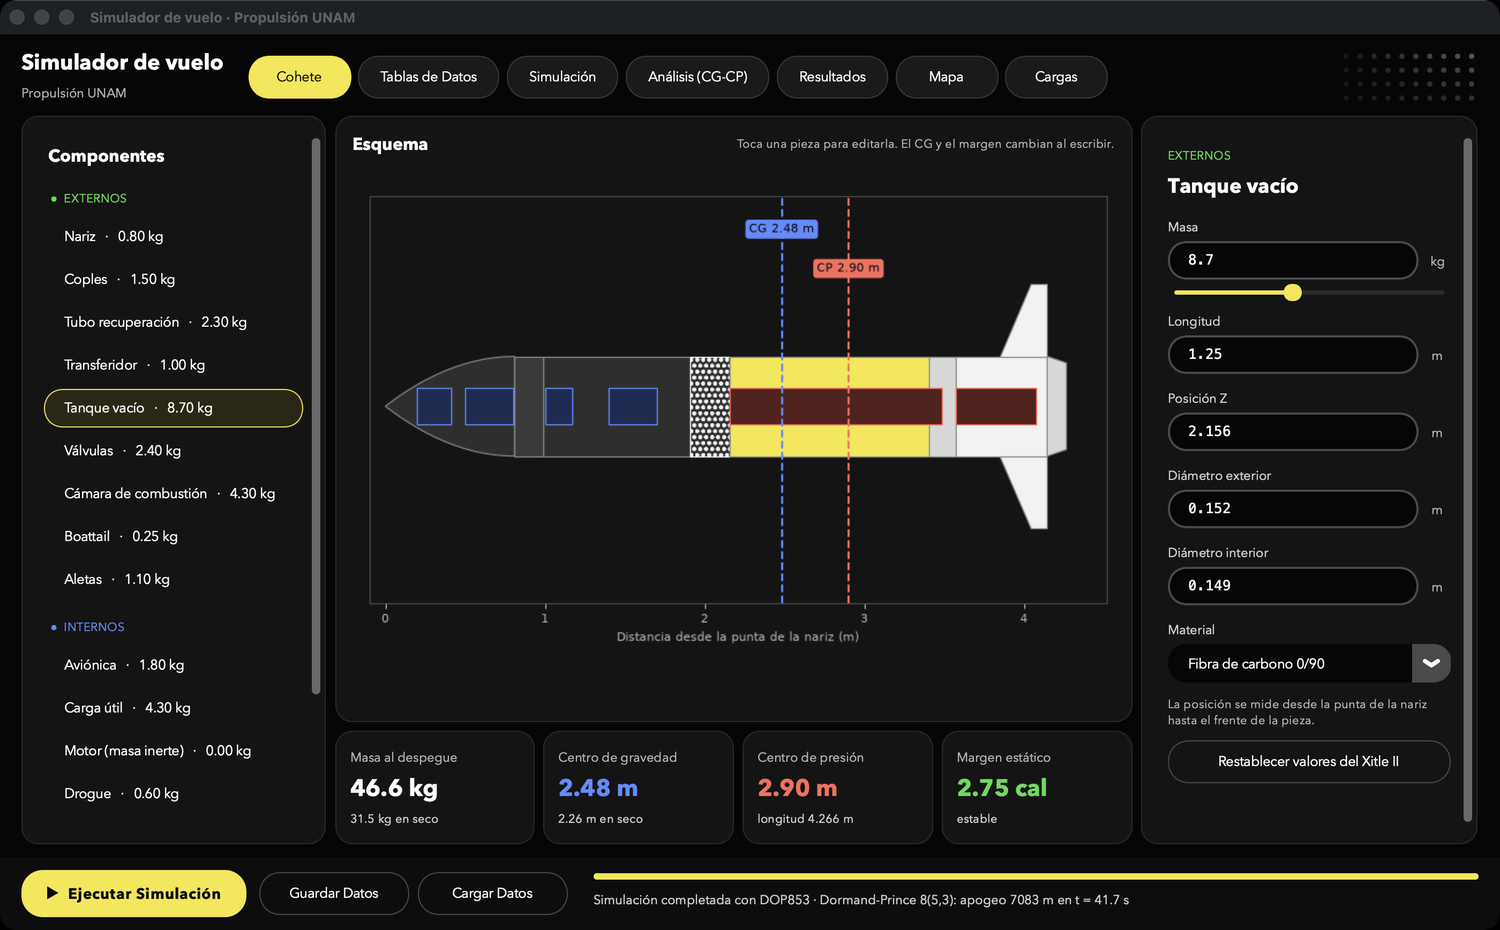
\includegraphics[keepaspectratio,alt={La
pestaña Cohete de la interfaz, con la lista de piezas, el
esquema y los campos de la pieza
elegida}]{figuras/propulsion-pestana-cohete.png}}
\caption{La pestaña Cohete de la interfaz, con la lista de
piezas, el esquema y los campos de la pieza elegida}
\end{figure}

\textbf{Reparto de la masa.} El propelente es el 34 \% de la
masa al despegue (15.85 kg). El tanque vacío, con 8.7 kg, es
la pieza estructural más pesada, casi el 28 \% de la masa
seca. La carga útil y la aviónica suman 6.1 kg en los
primeros 80 cm.

\textbf{Qué dice del diseño.} La masa pesada de adelante
(carga útil y aviónica) y el tanque al centro dejan el
centro de gravedad a 2.48 m, el 58 \% de la longitud. Eso
ayuda a la estabilidad sin necesidad de lastre. El oxidante
está casi sobre el centro de gravedad, así que al consumirse
cambia poco el equilibrio. El grano y la cámara están atrás,
y al quemarse el grano el centro de gravedad se mueve hacia
la nariz, de 2.48 a 2.26 m.

El momento de inercia transversal baja de 59.3 a 50.6 kg·m²
durante el quemado.

\section{El motor}\label{el-motor}

El empuje viene de la prueba estática del 28 de mayo de
2024.

{\def\LTcaptype{none} % do not increment counter
\begin{longtable}[]{@{}
  >{\raggedright\arraybackslash}p{(\linewidth - 2\tabcolsep) * \real{0.5000}}
  >{\raggedright\arraybackslash}p{(\linewidth - 2\tabcolsep) * \real{0.5000}}@{}}
\toprule\noalign{}
\begin{minipage}[b]{\linewidth}\raggedright
Cantidad
\end{minipage} & \begin{minipage}[b]{\linewidth}\raggedright
Valor
\end{minipage} \\
\midrule\noalign{}
\endhead
\bottomrule\noalign{}
\endlastfoot
Impulso total & 21 139 N·s \\
Duración & 21.6 s \\
Empuje máximo & 2390 N a los 2.4 s \\
Empuje medio en todo el quemado & 978 N \\
Empuje medio en los primeros 10 s & 1867 N \\
Propelente consumido & 15.07 kg (12.75 de oxidante, 2.32 de
grano) \\
Impulso específico & 143 s \\
Relación empuje a peso al despegue & 4.1 \\
\end{longtable}
}

\begin{figure}
\centering
\pandocbounded{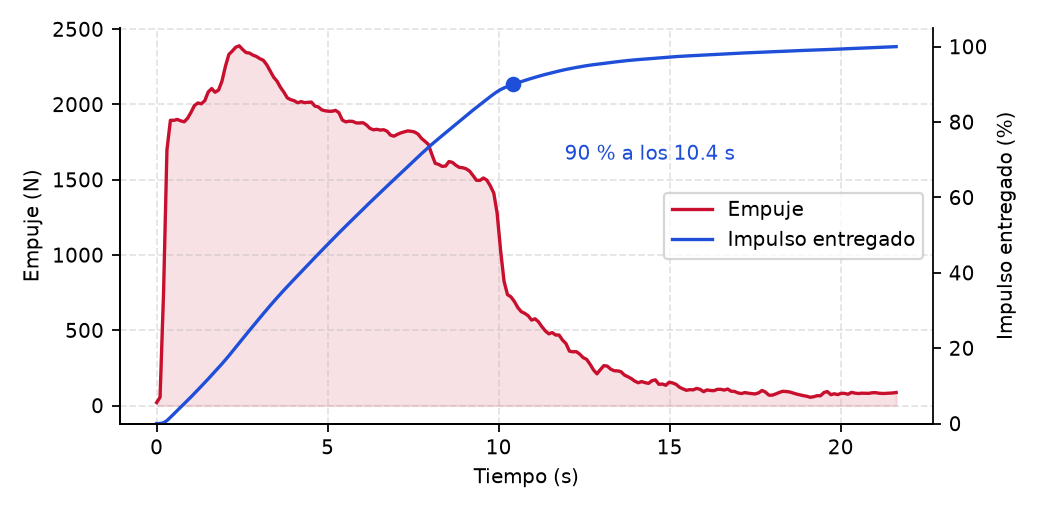
\includegraphics[keepaspectratio,alt={Curva
de empuje de la prueba estática e impulso
entregado}]{figuras/motor.png}}
\caption{Curva de empuje de la prueba estática e impulso
entregado}
\end{figure}

\textbf{Clase del motor.} Con 21 139 N·s el motor es de
clase O, apenas 3 \% arriba del límite entre N y O (20 480
N·s).

\textbf{Forma de la curva.} El empuje es regresivo. Sube a
2390 N en 2.4 s, se mantiene cerca de 1900 N hasta los 10 s
y cae. A los 5.3 s el motor ya entregó la mitad del impulso
y a los 10.4 s el 90 \%. De ahí hasta los 21.6 s queda una
cola de unos 80 a 100 N.

\textbf{Qué dice del diseño.} Esa cola no ayuda. Al final
del quemado el empuje es de 86 N, el arrastre de 105 N y el
peso de 309 N, así que el cohete ya va frenando. Es el
comportamiento de un tanque de óxido nitroso que se queda
sin líquido y termina expulsando gas. Para el vuelo, el
motor es en la práctica uno de 10 s.

La relación empuje a peso de 4.1 es cómoda para salir del
riel. La aceleración máxima es de 4.6 g a los 2.4 s, baja
para la electrónica y la carga útil.

\textbf{Impulso específico.} Los 143 s son pocos para un
híbrido de óxido nitroso. Hay que tomarlo con cuidado,
porque el impulso viene de la prueba estática y la masa
consumida de una simulación del motor que dura 10 s. Si las
dos tablas no corresponden al mismo motor, el número no
significa mucho. Vale la pena pesar el propelente antes y
después de una prueba.

\textbf{Velocidad ideal contra la real.} Con ese impulso y
esa masa, la ecuación del cohete da 548 m/s. El cohete
alcanza 343 m/s. Los 205 m/s que faltan se van en vencer la
gravedad y el arrastre durante el quemado.

\section{Estabilidad}\label{estabilidad}

{\def\LTcaptype{none} % do not increment counter
\begin{longtable}[]{@{}
  >{\raggedright\arraybackslash}p{(\linewidth - 4\tabcolsep) * \real{0.3333}}
  >{\raggedright\arraybackslash}p{(\linewidth - 4\tabcolsep) * \real{0.3333}}
  >{\raggedright\arraybackslash}p{(\linewidth - 4\tabcolsep) * \real{0.3333}}@{}}
\toprule\noalign{}
\begin{minipage}[b]{\linewidth}\raggedright
\end{minipage} & \begin{minipage}[b]{\linewidth}\raggedright
Al despegue
\end{minipage} & \begin{minipage}[b]{\linewidth}\raggedright
Sin propelente
\end{minipage} \\
\midrule\noalign{}
\endhead
\bottomrule\noalign{}
\endlastfoot
Centro de gravedad & 2.48 m & 2.26 m \\
Centro de presión & 2.90 m & 2.90 m \\
Margen estático & 2.75 calibres & 4.22 calibres \\
Distancia entre ambos & 0.42 m (9.8 \% de la longitud) &
0.64 m (15 \%) \\
\end{longtable}
}

\begin{figure}
\centering
\pandocbounded{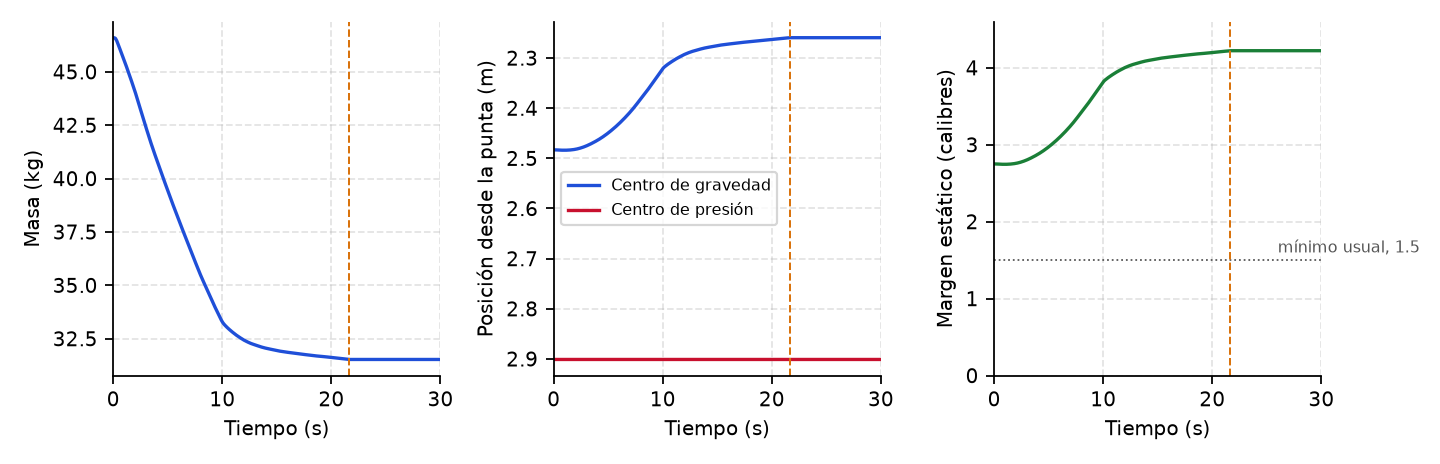
\includegraphics[keepaspectratio,alt={Masa,
centro de gravedad, centro de presión y margen estático
durante el quemado}]{figuras/estabilidad.png}}
\caption{Masa, centro de gravedad, centro de presión y
margen estático durante el quemado}
\end{figure}

El centro de presión sale de las fórmulas de Barrowman. Las
aletas aportan un coeficiente de fuerza normal de 5.26, la
nariz 2.00 y el boattail resta 0.49.

\textbf{Interpretación.} El cohete es estable porque el
centro de presión está detrás del centro de gravedad. Si el
viento lo desvía, la fuerza normal lo regresa. El margen se
mide en calibres, es decir, en diámetros del cohete. La
regla usual pide al menos 1.5.

En un cohete tan esbelto conviene ver también el margen como
fracción de la longitud. Los 2.75 calibres son el 9.8 \% del
largo, un valor normal. El número en calibres se ve alto
porque el diámetro es pequeño.

\textbf{Qué dice del diseño.}

\begin{itemize}
\tightlist
\item
  El margen crece durante el vuelo, de 2.75 a 4.22 calibres.
  Nunca baja del valor de despegue, que es la condición más
  exigente porque ahí el cohete va lento.
\item
  Hacia el final del quemado el cohete queda sobrado de
  estabilidad. Un cohete así gira con facilidad hacia el
  viento. Con 8 m/s de viento de frente el apogeo baja a
  6279 m, 11 \% menos.
\item
  Las aletas no están sobradas. Con tres aletas en lugar de
  cuatro el margen cae a 1.03 calibres. Con 9 cm de
  envergadura en lugar de 11 cae a 0.63. El tamaño actual es
  el que se necesita.
\item
  La carga útil importa. Con 2 kg menos adelante el margen
  baja a 2.18 calibres. Volar sin carga útil o con una más
  ligera pide revisar la estabilidad.
\end{itemize}

\textbf{Dos advertencias.}

La posición de las aletas la supuse. En el modelo, la raíz
termina donde empieza el boattail. Antes estaba 30 cm más
atrás y el margen salía de 4.24 calibres. El margen depende
mucho de esa medida, así que hay que tomarla del cohete
real.

Las fórmulas de Barrowman valen en régimen subsónico y con
ángulos de ataque pequeños. El cohete llega a Mach 1.01.
Cerca de Mach 1 el centro de presión real se mueve, y el
modelo no lo considera.

\section{El vuelo simulado}\label{el-vuelo-simulado}

\begin{figure}
\centering
\pandocbounded{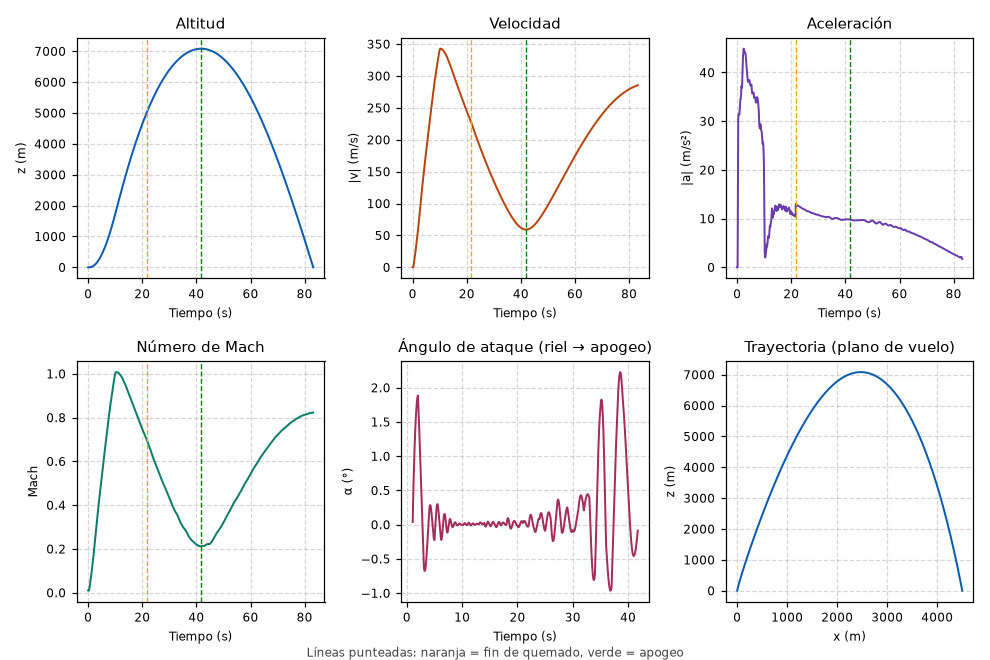
\includegraphics[keepaspectratio,alt={Altitud,
velocidad, aceleración, Mach, ángulo de ataque y trayectoria
del vuelo
simulado}]{figuras/resultados-vuelo.png}}
\caption{Altitud, velocidad, aceleración, Mach, ángulo de
ataque y trayectoria del vuelo simulado}
\end{figure}

{\def\LTcaptype{none} % do not increment counter
\begin{longtable}[]{@{}
  >{\raggedright\arraybackslash}p{(\linewidth - 10\tabcolsep) * \real{0.1667}}
  >{\raggedright\arraybackslash}p{(\linewidth - 10\tabcolsep) * \real{0.1667}}
  >{\raggedright\arraybackslash}p{(\linewidth - 10\tabcolsep) * \real{0.1667}}
  >{\raggedright\arraybackslash}p{(\linewidth - 10\tabcolsep) * \real{0.1667}}
  >{\raggedright\arraybackslash}p{(\linewidth - 10\tabcolsep) * \real{0.1667}}
  >{\raggedright\arraybackslash}p{(\linewidth - 10\tabcolsep) * \real{0.1667}}@{}}
\toprule\noalign{}
\begin{minipage}[b]{\linewidth}\raggedright
Instante
\end{minipage} & \begin{minipage}[b]{\linewidth}\raggedright
Tiempo (s)
\end{minipage} & \begin{minipage}[b]{\linewidth}\raggedright
Altura (m)
\end{minipage} & \begin{minipage}[b]{\linewidth}\raggedright
Velocidad (m/s)
\end{minipage} & \begin{minipage}[b]{\linewidth}\raggedright
Mach
\end{minipage} & \begin{minipage}[b]{\linewidth}\raggedright
Masa (kg)
\end{minipage} \\
\midrule\noalign{}
\endhead
\bottomrule\noalign{}
\endlastfoot
Salida del riel & 1.05 & 10 & 25.3 & 0.07 & 45.5 \\
Empuje máximo & 2.4 & 77 & 77 & 0.22 & 43.4 \\
Presión dinámica máxima & 10.1 & 1768 & 342 & 1.01 & 33.2 \\
Velocidad máxima & 10.4 & 1862 & 343 & 1.01 & 33.0 \\
Fin del quemado & 21.6 & 5007 & 228 & 0.70 & 31.5 \\
Apogeo & 41.7 & 7083 & 59 & 0.21 & 31.5 \\
Impacto (sin paracaídas) & 83.2 & 0 & 285 & 0.82 & 31.5 \\
\end{longtable}
}

\begin{figure}
\centering
\pandocbounded{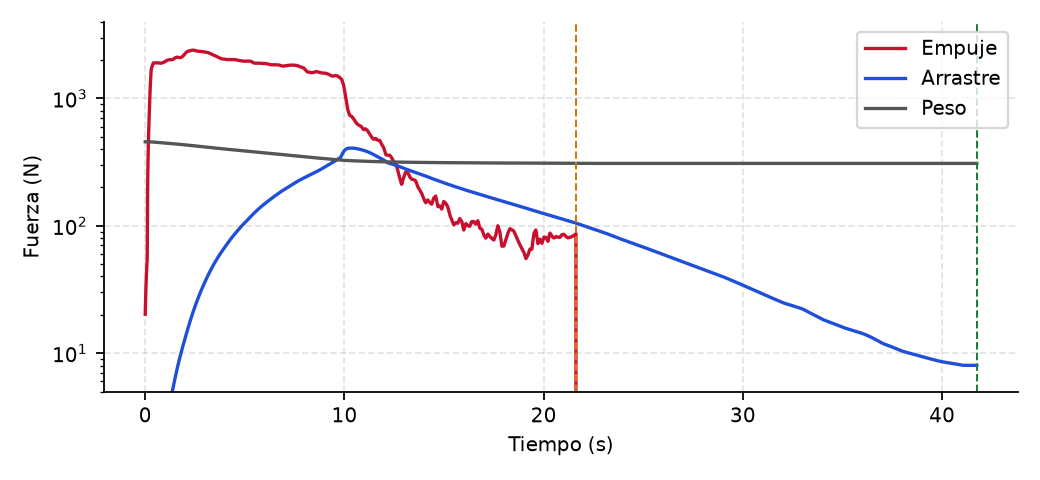
\includegraphics[keepaspectratio,alt={Empuje,
arrastre y peso durante el ascenso, en escala
logarítmica}]{figuras/fuerzas.png}}
\caption{Empuje, arrastre y peso durante el ascenso, en
escala logarítmica}
\end{figure}

La figura anterior compara las tres fuerzas. El empuje
domina hasta los 10 s. Después cae por debajo del peso y,
hacia el final del quemado, también por debajo del arrastre.

\textbf{En el riel.} El cohete recorre los 10 m del riel en
1.05 s y sale a 25.3 m/s. A esa velocidad las aletas ya
trabajan. Con un riel de 5 m saldría a 17.6 m/s, que es
justo. El riel de 10 m está bien elegido.

\textbf{Ascenso con motor.} La aceleración máxima es de 44.9
m/s² a los 2.4 s. La velocidad máxima, 343 m/s, llega a los
10.4 s, cuando el empuje cae. Ahí también ocurre la presión
dinámica máxima, 50.2 kPa a 1.77 km de altura. Es el momento
de mayor carga aerodinámica.

\textbf{El paso por Mach 1.} El coeficiente de arrastre sube
de 0.36 en subsónico a 0.45 en Mach 1.01. El arrastre máximo
es de 407 N. El cohete toca Mach 1 y no pasa de ahí, así que
vuela varios segundos en la zona donde el arrastre es mayor.
Con 5 \% menos de empuje se queda en Mach 0.95.

\textbf{Ascenso sin motor.} Del fin del quemado al apogeo el
cohete sube otros 2076 m en 20 s, solo con la velocidad que
lleva. El 29 \% de la altura se gana sin empuje.

\textbf{Apogeo.} A los 41.7 s el cohete está a 7083 m y a
2471 m de distancia horizontal. Todavía lleva 59 m/s, casi
todo horizontal, porque el riel está inclinado a 83°.

\textbf{Ángulo de ataque.} Se mantiene entre −1.0° y 2.2° en
todo el ascenso. Con el viento de ese día, de 1.5 m/s en
superficie, el cohete vuela casi alineado con el aire.

\begin{figure}
\centering
\pandocbounded{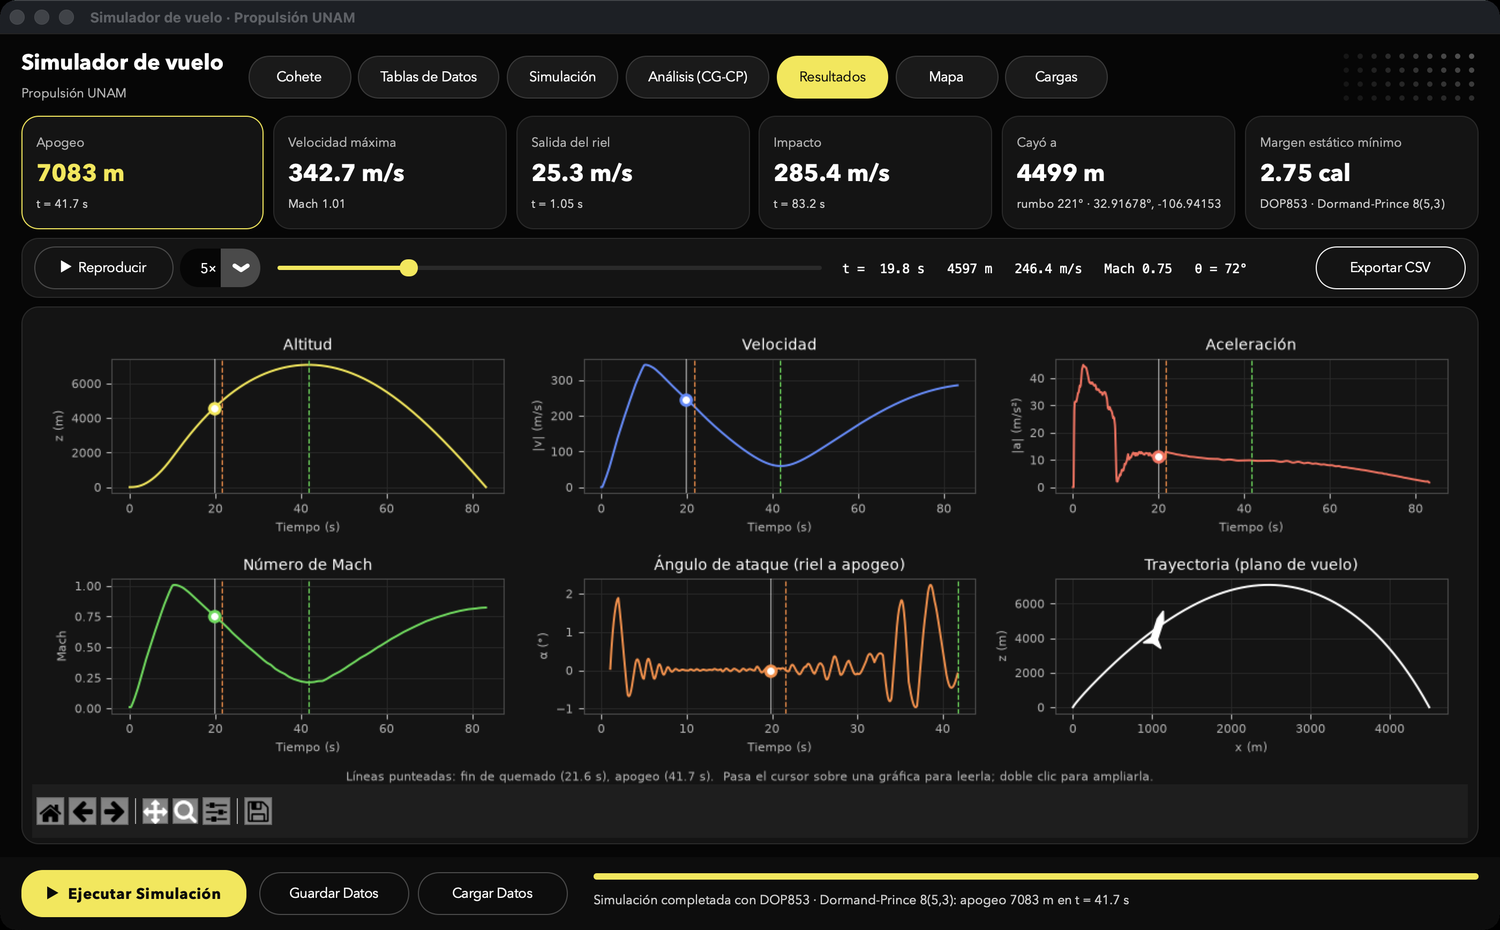
\includegraphics[keepaspectratio,alt={La
pestaña Resultados de la interfaz, con el vuelo detenido a
los 19.8
s}]{figuras/propulsion-pestana-resultados.png}}
\caption{La pestaña Resultados de la interfaz, con el vuelo
detenido a los 19.8 s}
\end{figure}

\textbf{Efecto de la altitud del sitio.} El sitio está a
1395 m y ese día hacía calor. El aire tenía una densidad de
1.01 kg/m³ contra los 1.225 del nivel del mar. Desde el
nivel del mar con atmósfera estándar el mismo cohete
llegaría a 6649 m, 434 m menos.

\section{Qué tanto cambia el
apogeo}\label{quuxe9-tanto-cambia-el-apogeo}

Cada renglón cambia una sola cosa respecto al caso base.

{\def\LTcaptype{none} % do not increment counter
\begin{longtable}[]{@{}
  >{\raggedright\arraybackslash}p{(\linewidth - 6\tabcolsep) * \real{0.2500}}
  >{\raggedright\arraybackslash}p{(\linewidth - 6\tabcolsep) * \real{0.2500}}
  >{\raggedright\arraybackslash}p{(\linewidth - 6\tabcolsep) * \real{0.2500}}
  >{\raggedright\arraybackslash}p{(\linewidth - 6\tabcolsep) * \real{0.2500}}@{}}
\toprule\noalign{}
\begin{minipage}[b]{\linewidth}\raggedright
Cambio
\end{minipage} & \begin{minipage}[b]{\linewidth}\raggedright
Apogeo (m)
\end{minipage} & \begin{minipage}[b]{\linewidth}\raggedright
Diferencia
\end{minipage} & \begin{minipage}[b]{\linewidth}\raggedright
Distancia de caída (m)
\end{minipage} \\
\midrule\noalign{}
\endhead
\bottomrule\noalign{}
\endlastfoot
Caso base & 7082 & & 4500 \\
Empuje −5 \% & 6592 & −490 & 4340 \\
Empuje +5 \% & 7389 & +307 & 4551 \\
Arrastre +10 \% & 6890 & −192 & 4310 \\
Arrastre +25 \% & 6608 & −474 & 4046 \\
Arrastre −10 \% & 7288 & +206 & 4708 \\
Carga útil +2 kg & 6715 & −367 & 4479 \\
Carga útil −2 kg & 7295 & +213 & 4401 \\
Riel a 80° & 6808 & −274 & 6154 \\
Riel a 85° & 7218 & +136 & 3290 \\
Riel a 87° & 7312 & +230 & 2004 \\
Riel a 90° & 7369 & +287 & 68 \\
Viento de 8 m/s cruzado & 7110 & +28 & 4424 \\
Viento de 8 m/s de frente & 6279 & −803 & 7673 \\
\end{longtable}
}

\begin{figure}
\centering
\pandocbounded{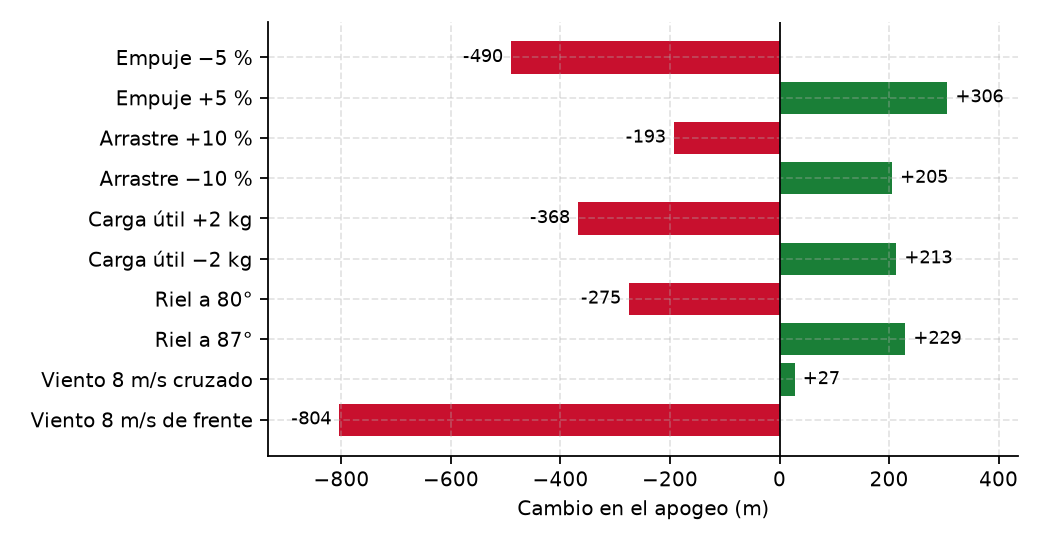
\includegraphics[keepaspectratio,alt={Cambio
del apogeo al variar un parámetro a la
vez}]{figuras/sensibilidad.png}}
\caption{Cambio del apogeo al variar un parámetro a la vez}
\end{figure}

\textbf{Qué dice del diseño.}

\begin{itemize}
\tightlist
\item
  \textbf{El empuje manda.} Un 5 \% de empuje vale unos 400
  m de apogeo, tanto como un 20 \% de arrastre. Conocer bien
  la curva de empuje importa más que afinar la tabla de
  arrastre.
\item
  \textbf{Cada kilogramo cuesta unos 150 m.} Es la
  referencia para decidir si vale la pena aligerar una
  pieza.
\item
  \textbf{El ángulo del riel casi no cambia el apogeo y
  cambia mucho dónde cae.} Entre 83° y 87° el apogeo sube
  230 m y la caída se acerca de 4.5 a 2.0 km. El ángulo se
  elige por la zona de recuperación.
\item
  \textbf{El viento de frente es el peor caso.} El cohete
  gira hacia el viento, vuela más tendido y pierde 800 m. El
  viento cruzado casi no afecta al apogeo.
\end{itemize}

\section{Recuperación}\label{recuperaciuxf3n}

{\def\LTcaptype{none} % do not increment counter
\begin{longtable}[]{@{}
  >{\raggedright\arraybackslash}p{(\linewidth - 6\tabcolsep) * \real{0.2500}}
  >{\raggedright\arraybackslash}p{(\linewidth - 6\tabcolsep) * \real{0.2500}}
  >{\raggedright\arraybackslash}p{(\linewidth - 6\tabcolsep) * \real{0.2500}}
  >{\raggedright\arraybackslash}p{(\linewidth - 6\tabcolsep) * \real{0.2500}}@{}}
\toprule\noalign{}
\begin{minipage}[b]{\linewidth}\raggedright
\end{minipage} & \begin{minipage}[b]{\linewidth}\raggedright
Vuelo libre
\end{minipage} & \begin{minipage}[b]{\linewidth}\raggedright
Solo drogue
\end{minipage} & \begin{minipage}[b]{\linewidth}\raggedright
Drogue y principal
\end{minipage} \\
\midrule\noalign{}
\endhead
\bottomrule\noalign{}
\endlastfoot
Velocidad de descenso a 3000 m & & 38 m/s & 38 m/s \\
Velocidad de impacto & 285 m/s & 33 m/s & 12.3 m/s \\
Tiempo de vuelo & 83 s & 228 s & 249 s \\
Distancia de caída & 4500 m & 2391 m & 2395 m \\
Fuerza de apertura del drogue & & 628 N (2.0 g) & 628 N (2.0
g) \\
Fuerza de apertura del principal & & & 1687 N (5.5 g) \\
\end{longtable}
}

\begin{figure}
\centering
\pandocbounded{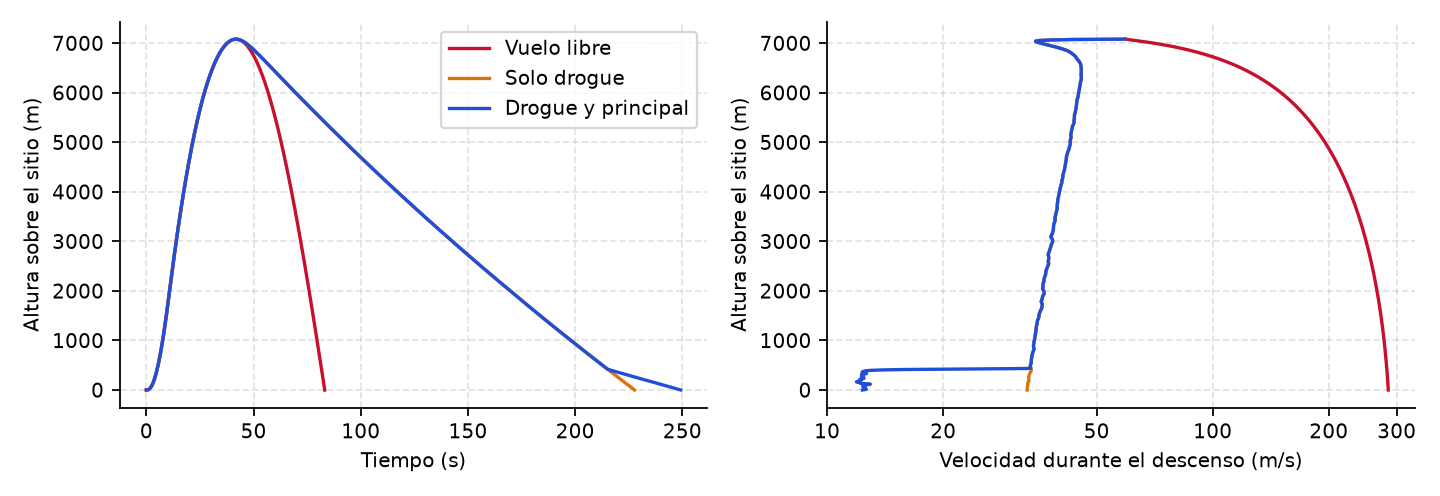
\includegraphics[keepaspectratio,alt={Altura
contra tiempo y velocidad de descenso con las tres opciones
de recuperación}]{figuras/recuperacion.png}}
\caption{Altura contra tiempo y velocidad de descenso con
las tres opciones de recuperación}
\end{figure}

El drogue tiene 0.944 m de diámetro y coeficiente de
arrastre de 0.8. El principal tiene 1.514 m y coeficiente de
2.0, y se abre a 450 m sobre el sitio.

\textbf{Interpretación.} El drogue se abre en el apogeo,
cuando el cohete va a 59 m/s, y lo estabiliza a 33 a 38 m/s.
Baja rápido a propósito para que el viento no lo arrastre
lejos. El principal se abre a baja altura y frena para el
aterrizaje.

\textbf{Qué dice del diseño.}

\begin{itemize}
\tightlist
\item
  \textbf{El principal es chico.} Aterrizar a 12.3 m/s
  equivale a caer desde 7.7 m de altura. Lo usual es buscar
  entre 5 y 9 m/s. Para llegar a 7 m/s con los 31.5 kg de
  masa seca haría falta un paracaídas de unos 2.7 m de
  diámetro con el mismo coeficiente.
\item
  \textbf{La apertura del principal es la carga más fuerte
  de la recuperación.} Son 1687 N, 5.5 veces el peso del
  cohete. Los herrajes y las cuerdas deben soportarla con
  margen.
\item
  \textbf{El drogue acerca el punto de caída.} Con
  paracaídas el cohete cae a 2.4 km del sitio y sin él a 4.5
  km, porque deja de avanzar al abrirse.
\item
  \textbf{Sin recuperación el cohete se pierde.} Llega al
  suelo a 285 m/s, Mach 0.82.
\end{itemize}

Las fuerzas de apertura dependen de la constante de llenado
de cada paracaídas, que es un valor supuesto.

\section{Análisis
estructural}\label{anuxe1lisis-estructural}

Esta sección responde a una pregunta: si el fuselaje y las
aletas aguantan las fuerzas del vuelo. Tiene cuatro partes.
Primero las cargas, luego el fuselaje, las aletas y la
recuperación. Al final hay dos comprobaciones que hice a
mano, fuera del simulador, y que marco como tales.

\subsection{Cómo se calculan las
cargas}\label{cuxf3mo-se-calculan-las-cargas}

El cohete se trata como una viga libre, sin apoyos. En cada
instante del ascenso se toman del simulador las fuerzas
externas y se colocan sobre la viga.

\begin{itemize}
\tightlist
\item
  El empuje entra por el extremo trasero.
\item
  El arrastre actúa en la punta de la nariz. Es el reparto
  más desfavorable para la compresión de los tramos
  delanteros.
\item
  La fuerza normal se reparte entre la nariz, las aletas y
  el boattail según su coeficiente, cada una en su centro de
  presión.
\item
  El peso de cada pieza se reparte a lo largo de su
  longitud.
\end{itemize}

Esas fuerzas aceleran al cohete. La aceleración produce
fuerzas de inercia sobre cada tramo, proporcionales a su
masa. Al cortar la viga en un punto y sumar todo lo que hay
de un lado, se obtiene lo que una mitad le hace a la otra.
De ahí salen tres cargas internas.

{\def\LTcaptype{none} % do not increment counter
\begin{longtable}[]{@{}
  >{\raggedright\arraybackslash}p{(\linewidth - 4\tabcolsep) * \real{0.3333}}
  >{\raggedright\arraybackslash}p{(\linewidth - 4\tabcolsep) * \real{0.3333}}
  >{\raggedright\arraybackslash}p{(\linewidth - 4\tabcolsep) * \real{0.3333}}@{}}
\toprule\noalign{}
\begin{minipage}[b]{\linewidth}\raggedright
Carga
\end{minipage} & \begin{minipage}[b]{\linewidth}\raggedright
Qué es
\end{minipage} & \begin{minipage}[b]{\linewidth}\raggedright
Qué hace sobre el tubo
\end{minipage} \\
\midrule\noalign{}
\endhead
\bottomrule\noalign{}
\endlastfoot
Compresión & fuerza a lo largo del eje & lo aplasta y puede
pandearlo \\
Cortante & fuerza transversal & tiende a cizallarlo \\
Momento flector & giro alrededor de un eje transversal & lo
dobla, comprime un lado y estira el otro \\
\end{longtable}
}

El análisis es cuasiestático. Supone que el cohete responde
como cuerpo rígido en cada instante. No incluye vibraciones.

\subsection{Los instantes más
exigentes}\label{los-instantes-muxe1s-exigentes}

{\def\LTcaptype{none} % do not increment counter
\begin{longtable}[]{@{}
  >{\raggedright\arraybackslash}p{(\linewidth - 10\tabcolsep) * \real{0.1667}}
  >{\raggedright\arraybackslash}p{(\linewidth - 10\tabcolsep) * \real{0.1667}}
  >{\raggedright\arraybackslash}p{(\linewidth - 10\tabcolsep) * \real{0.1667}}
  >{\raggedright\arraybackslash}p{(\linewidth - 10\tabcolsep) * \real{0.1667}}
  >{\raggedright\arraybackslash}p{(\linewidth - 10\tabcolsep) * \real{0.1667}}
  >{\raggedright\arraybackslash}p{(\linewidth - 10\tabcolsep) * \real{0.1667}}@{}}
\toprule\noalign{}
\begin{minipage}[b]{\linewidth}\raggedright
Instante
\end{minipage} & \begin{minipage}[b]{\linewidth}\raggedright
Tiempo (s)
\end{minipage} & \begin{minipage}[b]{\linewidth}\raggedright
Presión dinámica (Pa)
\end{minipage} & \begin{minipage}[b]{\linewidth}\raggedright
Mach
\end{minipage} & \begin{minipage}[b]{\linewidth}\raggedright
Compresión máxima (N)
\end{minipage} & \begin{minipage}[b]{\linewidth}\raggedright
Momento máximo (N·m)
\end{minipage} \\
\midrule\noalign{}
\endhead
\bottomrule\noalign{}
\endlastfoot
Salida del riel & 1.05 & 324 & 0.07 & 1968 & 0.0 \\
Empuje máximo & 2.4 & 3007 & 0.22 & 2387 & 2.6 \\
Momento máximo con el viento del día & 5.5 & 19 473 & 0.58 &
1887 & 4.6 \\
Presión dinámica máxima & 10.1 & 50 028 & 1.01 & 939 &
0.3 \\
Ráfaga lateral de 9 m/s & 10.5 & 50 000 & 1.01 & 939 & 57 \\
\end{longtable}
}

\textbf{Interpretación.} Hay dos momentos críticos y son
distintos. La compresión manda al principio, cuando el
empuje es máximo y el cohete está más pesado. La flexión
manda a los 10 s, cuando la presión dinámica es máxima,
porque cualquier ángulo de ataque produce ahí la mayor
fuerza lateral.

Con el viento del día el cohete vuela casi alineado con el
aire y la flexión es mínima, apenas 5 N·m. Ese día no es
representativo. Por eso se calcula un caso de diseño con una
ráfaga lateral de 9 m/s que llega de golpe, sin que el
cohete alcance a girar. La ráfaga da un ángulo de ataque de
1.5° y multiplica el momento por doce.

\subsection{Cargas a lo largo del
cohete}\label{cargas-a-lo-largo-del-cohete}

\begin{figure}
\centering
\pandocbounded{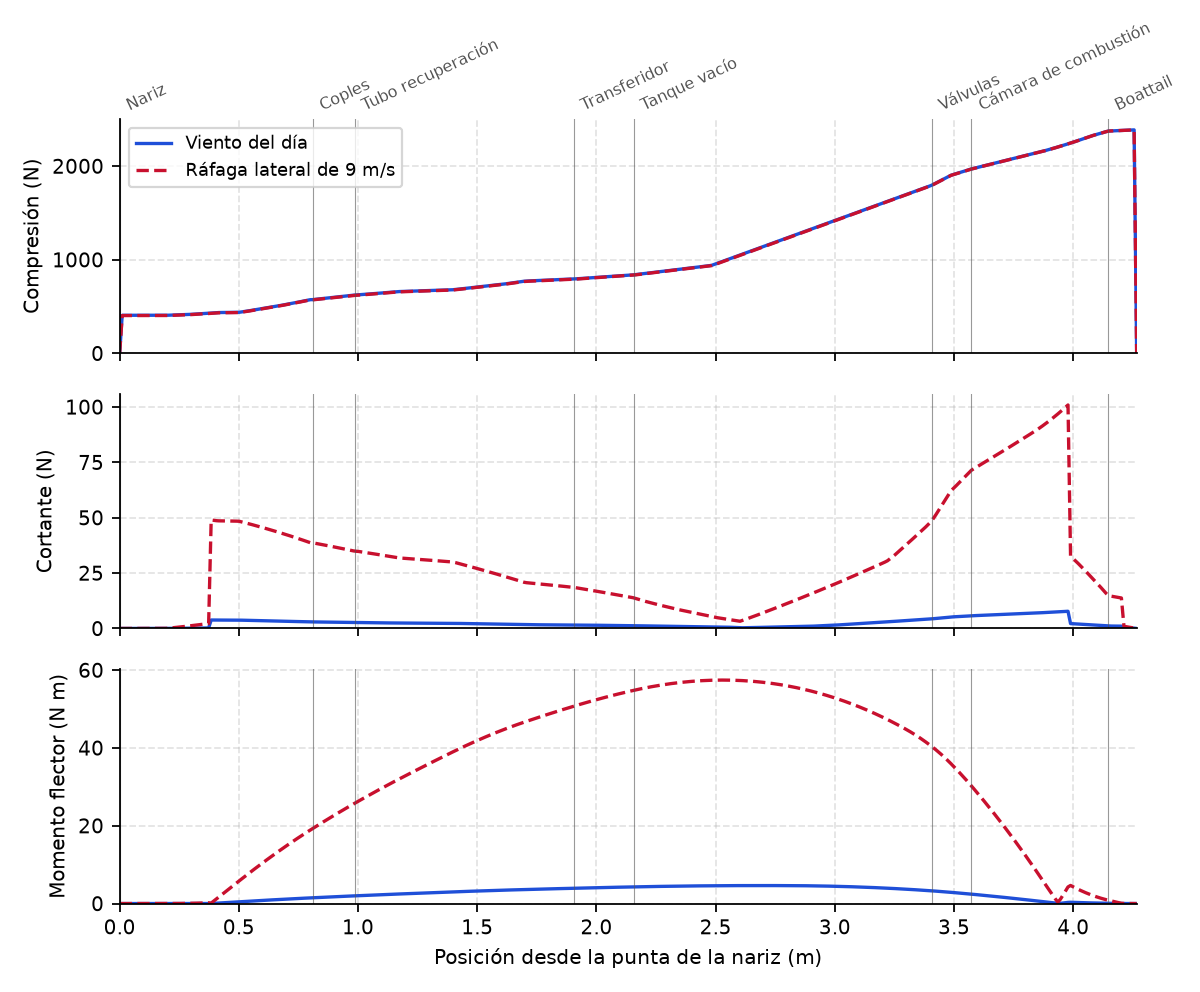
\includegraphics[keepaspectratio,alt={Compresión,
cortante y momento flector máximos en cada sección del
cohete durante el
ascenso}]{figuras/cargas.png}}
\caption{Compresión, cortante y momento flector máximos en
cada sección del cohete durante el ascenso}
\end{figure}

{\def\LTcaptype{none} % do not increment counter
\begin{longtable}[]{@{}
  >{\raggedright\arraybackslash}p{(\linewidth - 4\tabcolsep) * \real{0.3333}}
  >{\raggedright\arraybackslash}p{(\linewidth - 4\tabcolsep) * \real{0.3333}}
  >{\raggedright\arraybackslash}p{(\linewidth - 4\tabcolsep) * \real{0.3333}}@{}}
\toprule\noalign{}
\begin{minipage}[b]{\linewidth}\raggedright
Carga máxima
\end{minipage} & \begin{minipage}[b]{\linewidth}\raggedright
Con el viento del día
\end{minipage} & \begin{minipage}[b]{\linewidth}\raggedright
Con ráfaga lateral de 9 m/s
\end{minipage} \\
\midrule\noalign{}
\endhead
\bottomrule\noalign{}
\endlastfoot
Compresión & 2387 N junto a la cola, a los 2.4 s & igual \\
Cortante & 8 N & 101 N a 3.98 m de la punta \\
Momento flector & 5 N·m & 57 N·m a 2.53 m de la punta \\
\end{longtable}
}

\textbf{Cómo leer la figura.}

\begin{itemize}
\tightlist
\item
  \textbf{La compresión crece hacia la cola.} Cada sección
  empuja toda la masa que tiene delante, así que la que más
  carga es la última. Los 400 N que aparecen desde la punta
  son el arrastre. El tramo donde la curva sube más rápido
  es el tanque, porque ahí está la masa del oxidante.
\item
  \textbf{El cortante salta en dos puntos.} A 0.38 m está el
  centro de presión de la nariz y a 3.98 m el de las aletas.
  Son los dos lugares donde el aire empuja de lado. Entre
  ellos el cortante cambia poco a poco por la inercia de la
  masa.
\item
  \textbf{El momento es máximo cerca del centro.} La nariz y
  las aletas empujan en los extremos y la masa del centro se
  resiste. El cohete se dobla como una regla sostenida por
  las puntas. El máximo cae a 2.53 m, dentro del tanque.
\end{itemize}

\begin{figure}
\centering
\pandocbounded{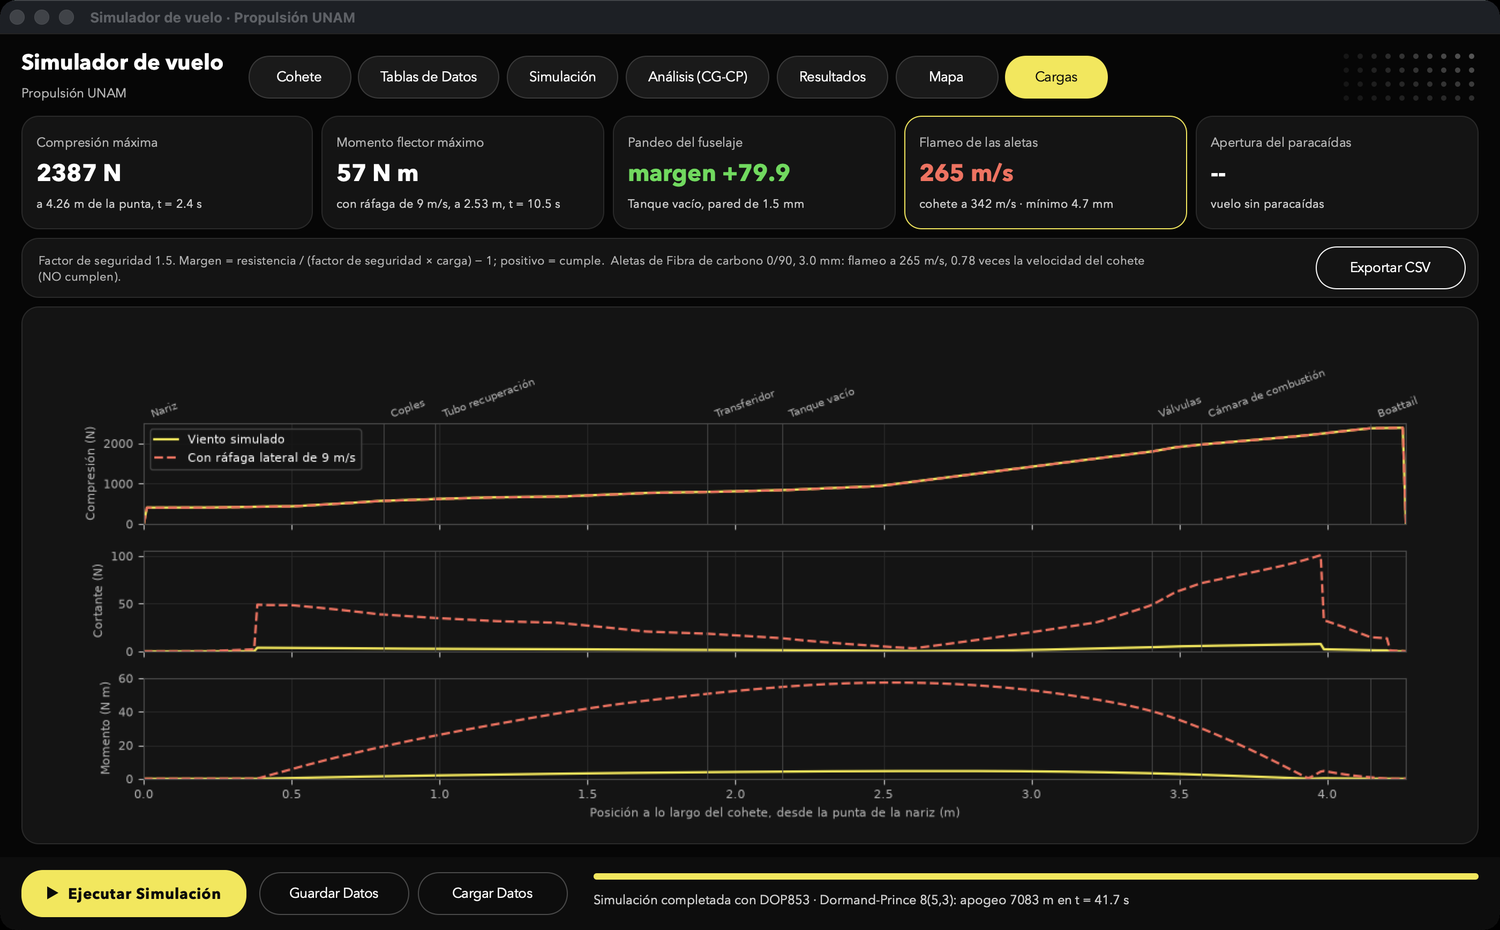
\includegraphics[keepaspectratio,alt={La
pestaña Cargas de la interfaz, con las tarjetas de
compresión, momento, pandeo y
flameo}]{figuras/propulsion-pestana-cargas.png}}
\caption{La pestaña Cargas de la interfaz, con las tarjetas
de compresión, momento, pandeo y flameo}
\end{figure}

\subsection{Fuselaje}\label{fuselaje}

Cada tramo cilíndrico se comprueba con la compresión y el
momento que soporta. La compresión se reparte en toda la
pared y da un esfuerzo axial. El momento da un esfuerzo de
flexión, máximo en el lado comprimido. Los dos se suman.

Un tubo de pared delgada falla por pandeo mucho antes de que
el material se rompa. La pared se arruga, como una lata al
pisarla. La fórmula clásica da el esfuerzo de pandeo de un
cilindro perfecto, y la monografía NASA SP-8007 da un factor
que lo reduce por las imperfecciones de un tubo real.

Para los tubos del Xitle II, con radio de 75 mm y pared de
1.5 mm:

{\def\LTcaptype{none} % do not increment counter
\begin{longtable}[]{@{}ll@{}}
\toprule\noalign{}
Cantidad & Valor \\
\midrule\noalign{}
\endhead
\bottomrule\noalign{}
\endlastfoot
Relación entre radio y espesor & 50 \\
Esfuerzo de pandeo clásico (fibra de carbono) & 810 MPa \\
Factor de reducción en compresión & 0.68 \\
Factor de reducción en flexión & 0.74 \\
Carga axial de pandeo & 389 kN \\
Factor de seguridad aplicado a las cargas & 1.5 \\
\end{longtable}
}

\begin{figure}
\centering
\pandocbounded{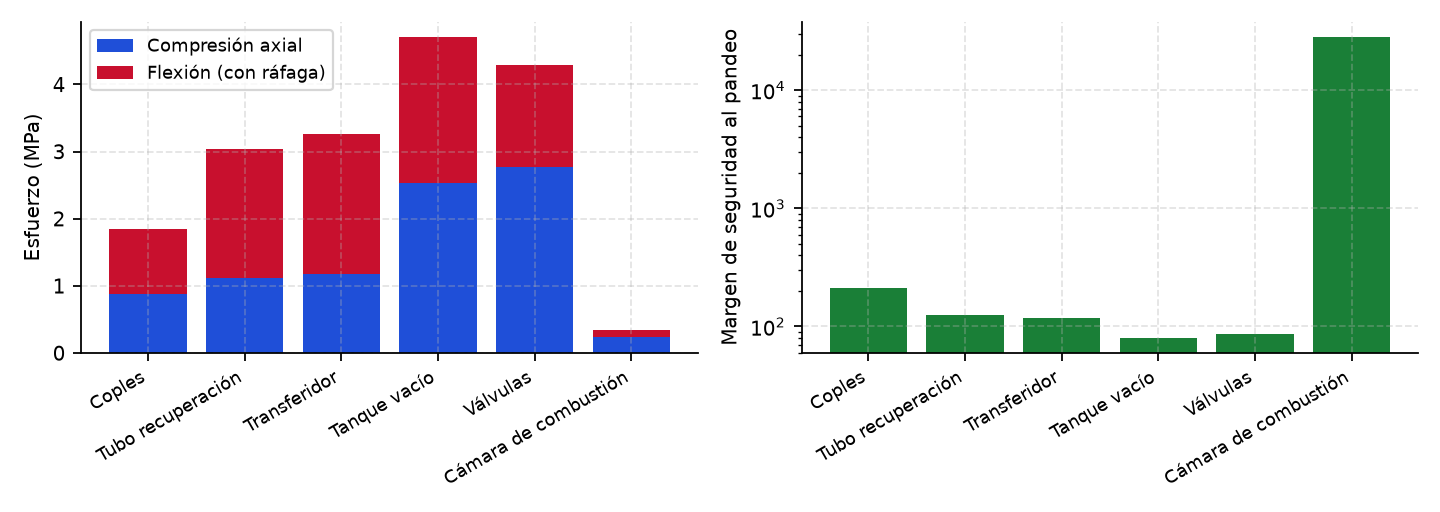
\includegraphics[keepaspectratio,alt={Esfuerzos
en cada tramo del fuselaje y margen de seguridad al
pandeo}]{figuras/esfuerzos.png}}
\caption{Esfuerzos en cada tramo del fuselaje y margen de
seguridad al pandeo}
\end{figure}

{\def\LTcaptype{none} % do not increment counter
\begin{longtable}[]{@{}
  >{\raggedright\arraybackslash}p{(\linewidth - 14\tabcolsep) * \real{0.1250}}
  >{\raggedright\arraybackslash}p{(\linewidth - 14\tabcolsep) * \real{0.1250}}
  >{\raggedright\arraybackslash}p{(\linewidth - 14\tabcolsep) * \real{0.1250}}
  >{\raggedright\arraybackslash}p{(\linewidth - 14\tabcolsep) * \real{0.1250}}
  >{\raggedright\arraybackslash}p{(\linewidth - 14\tabcolsep) * \real{0.1250}}
  >{\raggedright\arraybackslash}p{(\linewidth - 14\tabcolsep) * \real{0.1250}}
  >{\raggedright\arraybackslash}p{(\linewidth - 14\tabcolsep) * \real{0.1250}}
  >{\raggedright\arraybackslash}p{(\linewidth - 14\tabcolsep) * \real{0.1250}}@{}}
\toprule\noalign{}
\begin{minipage}[b]{\linewidth}\raggedright
Tramo
\end{minipage} & \begin{minipage}[b]{\linewidth}\raggedright
Material
\end{minipage} & \begin{minipage}[b]{\linewidth}\raggedright
Compresión (N)
\end{minipage} & \begin{minipage}[b]{\linewidth}\raggedright
Momento (N·m)
\end{minipage} & \begin{minipage}[b]{\linewidth}\raggedright
Esfuerzo axial (MPa)
\end{minipage} & \begin{minipage}[b]{\linewidth}\raggedright
Esfuerzo de flexión (MPa)
\end{minipage} & \begin{minipage}[b]{\linewidth}\raggedright
Margen al pandeo
\end{minipage} & \begin{minipage}[b]{\linewidth}\raggedright
Margen de resistencia
\end{minipage} \\
\midrule\noalign{}
\endhead
\bottomrule\noalign{}
\endlastfoot
Coples & aluminio 6061-T6 & 622 & 25.6 & 0.88 & 0.97 & +214
& +99 \\
Tubo de recuperación & fibra de carbono & 794 & 50.6 & 1.12
& 1.92 & +126 & +124 \\
Transferidor & fibra de carbono & 839 & 54.8 & 1.18 & 2.07 &
+118 & +116 \\
Tanque & fibra de carbono & 1792 & 57.4 & 2.53 & 2.17 & +80
& +80 \\
Válvulas & fibra de carbono & 1970 & 40.1 & 2.78 & 1.52 &
+87 & +87 \\
Cámara de combustión & fibra de carbono & 2369 & 29.5 & 0.24
& 0.11 & más de +1000 & más de +1000 \\
\end{longtable}
}

El margen es la resistencia dividida entre la carga
multiplicada por el factor de seguridad, menos uno. Un
margen positivo significa que cumple. Un margen de +80
significa que el tramo aguantaría 81 veces la carga de
diseño.

\textbf{Interpretación.} El tramo más exigido es el tanque.
Tiene mucha compresión por estar atrás y el momento máximo
por estar al centro. Aun así trabaja a 4.7 MPa, cuando el
pandeo llegaría cerca de 550 MPa. La flexión de la ráfaga
pesa tanto como la compresión del empuje en los tramos
delanteros, y en el tanque los dos efectos son casi iguales.

La cámara de combustión tiene una pared de 25 mm en el
modelo, y por eso sus esfuerzos son diez veces menores.

\textbf{Qué dice del diseño.} Las cargas de vuelo no
dimensionan el fuselaje. Un tubo con la tercera parte de la
pared seguiría cumpliendo por pandeo. Lo que define los
espesores es otra cosa. En el tanque es la presión interna.
En los demás tubos son la fabricación, las uniones y el
manejo en tierra.

\subsection{Aletas}\label{aletas}

El flameo es una vibración de la aleta que se alimenta del
aire. A cierta velocidad, la torsión y la flexión de la
aleta se acoplan y la oscilación crece hasta romperla en una
fracción de segundo. La velocidad a la que empieza depende
de la rigidez a torsión del material, del espesor, de la
forma de la aleta y de la presión del aire.

Las aletas del Xitle II tienen 11 cm de envergadura, cuerda
de raíz de 30 cm, cuerda de punta de 10 cm y 3 mm de
espesor. El espesor es el 1 \% de la cuerda de raíz. El
material es fibra de carbono tejida a 0/90, con un módulo de
cortante de 5 GPa.

\begin{figure}
\centering
\pandocbounded{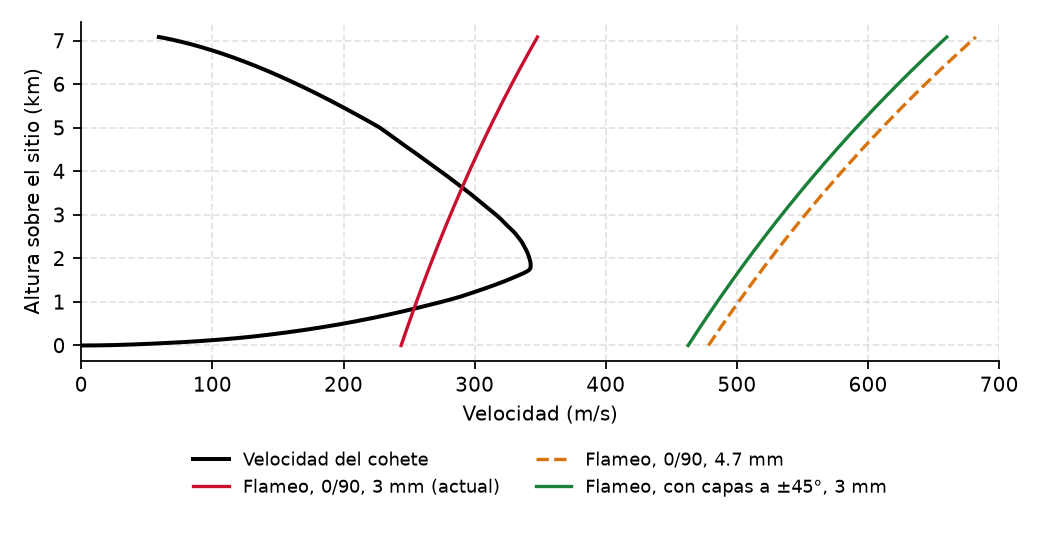
\includegraphics[keepaspectratio,alt={Velocidad
del cohete durante el ascenso y velocidad de flameo de las
aletas con tres
configuraciones}]{figuras/flameo.png}}
\caption{Velocidad del cohete durante el ascenso y velocidad
de flameo de las aletas con tres configuraciones}
\end{figure}

{\def\LTcaptype{none} % do not increment counter
\begin{longtable}[]{@{}
  >{\raggedright\arraybackslash}p{(\linewidth - 4\tabcolsep) * \real{0.3333}}
  >{\raggedright\arraybackslash}p{(\linewidth - 4\tabcolsep) * \real{0.3333}}
  >{\raggedright\arraybackslash}p{(\linewidth - 4\tabcolsep) * \real{0.3333}}@{}}
\toprule\noalign{}
\begin{minipage}[b]{\linewidth}\raggedright
Configuración
\end{minipage} & \begin{minipage}[b]{\linewidth}\raggedright
Velocidad de flameo a 1.77 km
\end{minipage} & \begin{minipage}[b]{\linewidth}\raggedright
Cociente con la velocidad del cohete
\end{minipage} \\
\midrule\noalign{}
\endhead
\bottomrule\noalign{}
\endlastfoot
0/90 con 3 mm (actual) & 265 m/s & 0.78 \\
0/90 con 4.7 mm & 520 m/s & 1.52 \\
Con capas a ±45° y 3 mm & 503 m/s & 1.47 \\
\end{longtable}
}

\textbf{Interpretación.} La velocidad de flameo sube con la
altura porque el aire es menos denso. La del cohete sube
mucho más rápido al principio. Las dos curvas se cruzan. El
cohete va por encima de la velocidad de flameo entre los 7 y
los 16 s de vuelo, de los 840 a los 3600 m de altura. Son
nueve segundos.

El tejido a 0/90 es rígido a lo largo y a lo ancho de la
aleta, pero blando a torsión, porque ninguna fibra va en
diagonal. La torsión es justo lo que gobierna el flameo.

\textbf{Qué dice del diseño.} Es el punto débil que señala
el análisis. Hay dos salidas y dan casi el mismo resultado.

\begin{itemize}
\tightlist
\item
  Subir el espesor a 4.7 mm. La velocidad de flameo crece
  con el espesor elevado a 1.5. El costo es un 57 \% más de
  masa en las aletas, unos 0.6 kg en la cola, que además
  mueven el centro de gravedad hacia atrás.
\item
  Agregar capas a ±45°. El módulo de cortante sube a unos 18
  GPa con los mismos 3 mm y la misma masa.
\end{itemize}

La segunda opción es mejor. No cuesta masa ni estabilidad.

\textbf{Cautelas.} Hay que leer esto como una alerta y no
como un veredicto.

\begin{itemize}
\tightlist
\item
  Las propiedades del material son de catálogo, no del
  laminado real.
\item
  La fórmula viene de NACA TN 4197 y es una estimación para
  aletas delgadas.
\item
  Existe otra forma de la misma fórmula, muy usada, que da
  una velocidad 41 \% mayor. Con ella el flameo empieza a
  375 m/s y el cociente es 1.10. Cumpliría sin el factor de
  seguridad y por poco.
\item
  El cohete voló el 22 de junio de 2024 con rumbo constante
  de principio a fin. Si hubiera perdido una aleta en el
  ascenso, la trayectoria se habría desviado. Los datos no
  muestran eso.
\end{itemize}

Lo que corresponde es medir el módulo de cortante del
laminado real y repetir la cuenta.

\subsection{Cargas de la
recuperación}\label{cargas-de-la-recuperaciuxf3n}

{\def\LTcaptype{none} % do not increment counter
\begin{longtable}[]{@{}lll@{}}
\toprule\noalign{}
Evento & Fuerza & En veces el peso \\
\midrule\noalign{}
\endhead
\bottomrule\noalign{}
\endlastfoot
Apertura del drogue en el apogeo & 628 N & 2.0 \\
Apertura del principal a 450 m & 1687 N & 5.5 \\
Empuje máximo, como referencia & 2390 N & 5.2 \\
\end{longtable}
}

\textbf{Interpretación.} La apertura del principal es una
carga del mismo orden que el empuje máximo. La diferencia es
el sentido. El empuje comprime el fuselaje. El paracaídas lo
jala y lo pone en tracción.

Repartida en la pared del tubo de recuperación, esa fuerza
da solo 2.4 MPa. El tubo no es el problema. La carga entra
por un punto, el herraje donde se amarra la cuerda, y ahí se
concentra. Lo que hay que dimensionar con esos 1687 N son el
herraje, su unión al fuselaje, la cuerda y las costuras del
paracaídas. Con el factor de seguridad de 1.5 son 2530 N.

Estas fuerzas dependen de la constante de llenado de cada
paracaídas, que es un valor supuesto. Un paracaídas que se
infla más rápido da una fuerza mayor.

\subsection{Dos comprobaciones fuera del
simulador}\label{dos-comprobaciones-fuera-del-simulador}

Estas dos cuentas las hice a mano con los datos del modelo.
No salen del programa.

\textbf{Presión del tanque.} El óxido nitroso se guarda como
líquido a su presión de vapor, que ronda los 51 bar a 20 °C
y los 63 bar a 30 °C. El día del vuelo hubo 30 °C. La
presión estira la pared a lo largo de la circunferencia. En
un tubo de 1.5 mm de pared y 75 mm de radio, ese esfuerzo es
de 250 a 310 MPa.

Eso es unas cien veces el esfuerzo que producen las cargas
de vuelo en el mismo tramo. Confirma que el tanque se
dimensiona por presión. También dice que la pared de 1.5 mm
que usa el modelo no es la del tanque real, porque con ella
quedaría poco margen para un recipiente a presión.

\textbf{Espesor que sugieren las masas.} El modelo toma el
espesor de pared de los diámetros, que dan 1.5 mm en todos
los tubos. Las masas cuentan otra historia.

{\def\LTcaptype{none} % do not increment counter
\begin{longtable}[]{@{}
  >{\raggedright\arraybackslash}p{(\linewidth - 6\tabcolsep) * \real{0.2500}}
  >{\raggedright\arraybackslash}p{(\linewidth - 6\tabcolsep) * \real{0.2500}}
  >{\raggedright\arraybackslash}p{(\linewidth - 6\tabcolsep) * \real{0.2500}}
  >{\raggedright\arraybackslash}p{(\linewidth - 6\tabcolsep) * \real{0.2500}}@{}}
\toprule\noalign{}
\begin{minipage}[b]{\linewidth}\raggedright
Tramo
\end{minipage} & \begin{minipage}[b]{\linewidth}\raggedright
Masa (kg)
\end{minipage} & \begin{minipage}[b]{\linewidth}\raggedright
Longitud (m)
\end{minipage} & \begin{minipage}[b]{\linewidth}\raggedright
Espesor que daría esa masa
\end{minipage} \\
\midrule\noalign{}
\endhead
\bottomrule\noalign{}
\endlastfoot
Tubo de recuperación & 2.3 & 0.92 & 3.3 mm de fibra de
carbono \\
Transferidor & 1.0 & 0.25 & 5.3 mm de fibra de carbono \\
Tanque & 8.7 & 1.25 & 9.2 mm de fibra de carbono o 5.4 mm de
aluminio \\
\end{longtable}
}

Las masas incluyen tapas, anillos y herrajes, así que el
espesor real de pared es menor que el de la tabla. Aun así,
las piezas pesan entre dos y seis veces lo que pesaría un
tubo de 1.5 mm.

\textbf{Qué dice del diseño.} Los márgenes de pandeo de esta
sección son conservadores si las paredes reales son más
gruesas. Y hay masa estructural que las cargas de vuelo no
justifican. Antes de aligerar hay que saber qué la
justifica: la presión, las uniones o la fabricación. El
tanque, con 8.7 kg, es donde más hay que ganar.

\subsection{Qué no cubre este
análisis}\label{quuxe9-no-cubre-este-anuxe1lisis}

\begin{itemize}
\tightlist
\item
  La presión interna del tanque y de la cámara de
  combustión, salvo la estimación anterior.
\item
  Las uniones entre tramos, los tornillos y los coples. En
  cohetes de este tipo suelen fallar antes que los tubos.
\item
  La unión de las aletas al fuselaje y la flexión de la
  aleta por la fuerza normal.
\item
  Vibraciones, golpes de encendido y cargas de transporte.
\item
  El impacto al aterrizar.
\item
  El calentamiento. A Mach 1 es pequeño, pero la cámara de
  combustión trabaja caliente.
\item
  El carácter ortótropo de la fibra de carbono. El pandeo se
  calcula como si el material fuera isótropo.
\end{itemize}

\section{El vuelo del 22 de junio de
2024}\label{el-vuelo-del-22-de-junio-de-2024}

El Xitle II voló en Spaceport America, Nuevo México, hacia
las 12:20 hora local. Los registros del rastreador GPS están
fechados el 22 de junio de 2024.

\subsection{Qué se midió}\label{quuxe9-se-midiuxf3}

{\def\LTcaptype{none} % do not increment counter
\begin{longtable}[]{@{}
  >{\raggedright\arraybackslash}p{(\linewidth - 2\tabcolsep) * \real{0.5000}}
  >{\raggedright\arraybackslash}p{(\linewidth - 2\tabcolsep) * \real{0.5000}}@{}}
\toprule\noalign{}
\begin{minipage}[b]{\linewidth}\raggedright
Registro
\end{minipage} & \begin{minipage}[b]{\linewidth}\raggedright
Contenido
\end{minipage} \\
\midrule\noalign{}
\endhead
\bottomrule\noalign{}
\endlastfoot
Rastreador GPS Featherweight & 74 puntos durante el vuelo,
uno por segundo, con posición, altura y velocidad \\
Telemetría ASYB & altura, presión, temperatura y
aceleraciones \\
Curva de altura contra tiempo & la altura cada segundo \\
\end{longtable}
}

{\def\LTcaptype{none} % do not increment counter
\begin{longtable}[]{@{}
  >{\raggedright\arraybackslash}p{(\linewidth - 2\tabcolsep) * \real{0.5000}}
  >{\raggedright\arraybackslash}p{(\linewidth - 2\tabcolsep) * \real{0.5000}}@{}}
\toprule\noalign{}
\begin{minipage}[b]{\linewidth}\raggedright
Cantidad medida
\end{minipage} & \begin{minipage}[b]{\linewidth}\raggedright
Valor
\end{minipage} \\
\midrule\noalign{}
\endhead
\bottomrule\noalign{}
\endlastfoot
Apogeo sobre el sitio & 6573 m (GPS) y 6569 m (curva de
altura) \\
Tiempo al apogeo & 42 s \\
Velocidad vertical máxima & 282 m/s a los 14 s, a 2577 m de
altura \\
Rumbo de la trayectoria & 220° \\
Distancia horizontal en el apogeo & 2532 m \\
Último punto GPS & a los 80 s, a 399 m de altura y 4553 m
del sitio \\
Velocidad en el último punto & 273 m/s hacia abajo \\
\end{longtable}
}

\textbf{El cohete bajó sin paracaídas.} El último punto lo
muestra a 399 m de altura cayendo a 273 m/s. La velocidad
vertical creció sin interrupción desde el apogeo, sin el
frenado que produciría un paracaídas. El sistema de
recuperación no actuó. Con los datos del repositorio no
puedo decir por qué.

\subsection{Condiciones del
día}\label{condiciones-del-duxeda}

{\def\LTcaptype{none} % do not increment counter
\begin{longtable}[]{@{}
  >{\raggedright\arraybackslash}p{(\linewidth - 2\tabcolsep) * \real{0.5000}}
  >{\raggedright\arraybackslash}p{(\linewidth - 2\tabcolsep) * \real{0.5000}}@{}}
\toprule\noalign{}
\begin{minipage}[b]{\linewidth}\raggedright
Dato
\end{minipage} & \begin{minipage}[b]{\linewidth}\raggedright
Valor
\end{minipage} \\
\midrule\noalign{}
\endhead
\bottomrule\noalign{}
\endlastfoot
Sitio & 32.94753° N, 106.91019° O, a 1395 m sobre el nivel
del mar \\
Temperatura en superficie & 29.8 °C, unos 20 °C arriba de la
atmósfera estándar \\
Presión en el sitio & 868.5 hPa \\
Viento en superficie & 1.5 m/s del oeste-noroeste \\
Viento en altura & 3.3 m/s a 5.9 km y 7.4 m/s a 7.7 km, del
suroeste \\
Riel & azimut de 220°, elevación de 83° \\
\end{longtable}
}

Los datos del tiempo son de modelo (reanálisis ERA5), no
mediciones en la plataforma. El ángulo del riel no quedó
registrado. Los 83° son el valor que reproduce la
trayectoria GPS.

\subsection{Simulación contra
medición}\label{simulaciuxf3n-contra-mediciuxf3n}

\begin{figure}
\centering
\pandocbounded{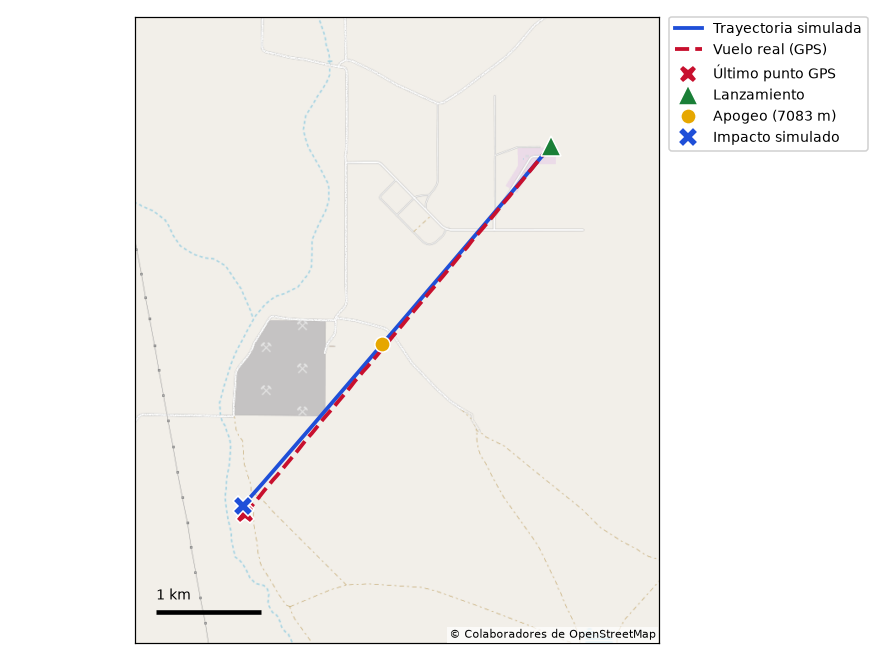
\includegraphics[keepaspectratio,alt={Trayectoria
simulada y trayectoria GPS del vuelo real sobre el
mapa}]{figuras/mapa-vuelo.png}}
\caption{Trayectoria simulada y trayectoria GPS del vuelo
real sobre el mapa}
\end{figure}

{\def\LTcaptype{none} % do not increment counter
\begin{longtable}[]{@{}
  >{\raggedright\arraybackslash}p{(\linewidth - 4\tabcolsep) * \real{0.3333}}
  >{\raggedright\arraybackslash}p{(\linewidth - 4\tabcolsep) * \real{0.3333}}
  >{\raggedright\arraybackslash}p{(\linewidth - 4\tabcolsep) * \real{0.3333}}@{}}
\toprule\noalign{}
\begin{minipage}[b]{\linewidth}\raggedright
\end{minipage} & \begin{minipage}[b]{\linewidth}\raggedright
Medido
\end{minipage} & \begin{minipage}[b]{\linewidth}\raggedright
Simulado
\end{minipage} \\
\midrule\noalign{}
\endhead
\bottomrule\noalign{}
\endlastfoot
Apogeo sobre el sitio & 6573 m & 7083 m \\
Tiempo al apogeo & 42 s & 41.7 s \\
Distancia horizontal en el apogeo & 2532 m & 2471 m \\
Rumbo & 220° & 221° \\
Velocidad al pasar por 399 m de altura & 273 m/s & 283
m/s \\
Punto final & 4553 m del sitio (aún en el aire) & 4499 m
(impacto) \\
\end{longtable}
}

La trayectoria sobre el terreno coincide. El impacto
simulado queda a 86 m del último punto GPS. No es una
predicción independiente, porque el ángulo del riel se
ajustó para eso.

El apogeo simulado es 510 m mayor, un 7.8 \%.

\subsection{Dónde aparece la
diferencia}\label{duxf3nde-aparece-la-diferencia}

Comparé la altura y la velocidad vertical segundo a segundo.

{\def\LTcaptype{none} % do not increment counter
\begin{longtable}[]{@{}
  >{\raggedright\arraybackslash}p{(\linewidth - 8\tabcolsep) * \real{0.2000}}
  >{\raggedright\arraybackslash}p{(\linewidth - 8\tabcolsep) * \real{0.2000}}
  >{\raggedright\arraybackslash}p{(\linewidth - 8\tabcolsep) * \real{0.2000}}
  >{\raggedright\arraybackslash}p{(\linewidth - 8\tabcolsep) * \real{0.2000}}
  >{\raggedright\arraybackslash}p{(\linewidth - 8\tabcolsep) * \real{0.2000}}@{}}
\toprule\noalign{}
\begin{minipage}[b]{\linewidth}\raggedright
Tiempo (s)
\end{minipage} & \begin{minipage}[b]{\linewidth}\raggedright
Altura medida (m)
\end{minipage} & \begin{minipage}[b]{\linewidth}\raggedright
Altura simulada (m)
\end{minipage} & \begin{minipage}[b]{\linewidth}\raggedright
Velocidad vertical medida (m/s)
\end{minipage} & \begin{minipage}[b]{\linewidth}\raggedright
Velocidad vertical simulada (m/s)
\end{minipage} \\
\midrule\noalign{}
\endhead
\bottomrule\noalign{}
\endlastfoot
5 & 458 & 414 & 158 & 180 \\
10 & 1495 & 1728 & 244 & 333 \\
15 & 2860 & 3326 & 279 & 294 \\
20 & 4169 & 4643 & 236 & 234 \\
30 & 5913 & 6397 & 118 & 119 \\
40 & 6562 & 7068 & 16 & 17 \\
50 & 6231 & 6754 & −80 & −79 \\
60 & 4989 & 5513 & −166 & −167 \\
70 & 2965 & 3481 & −234 & −236 \\
80 & 399 & 894 & −273 & −277 \\
\end{longtable}
}

\begin{figure}
\centering
\pandocbounded{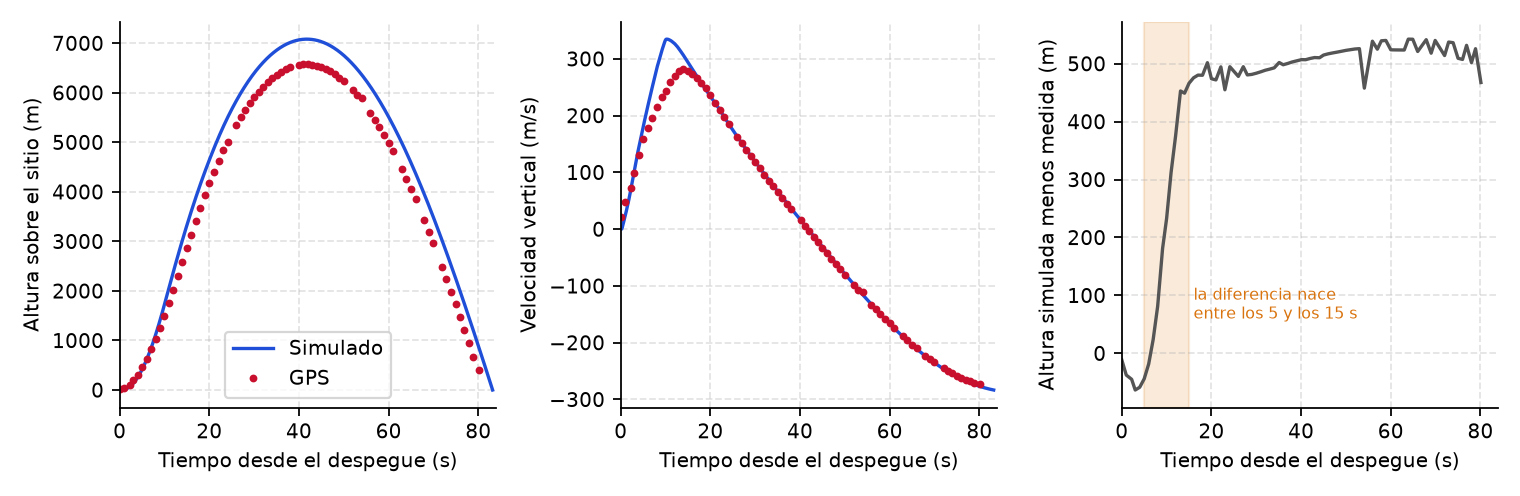
\includegraphics[keepaspectratio,alt={Altura
y velocidad vertical simuladas y medidas, y la diferencia de
altura entre ambas}]{figuras/vuelo-real.png}}
\caption{Altura y velocidad vertical simuladas y medidas, y
la diferencia de altura entre ambas}
\end{figure}

\textbf{Lo que se ve.}

\begin{itemize}
\tightlist
\item
  De los 20 s en adelante la velocidad simulada y la medida
  coinciden con diferencias de 1 a 4 m/s, en el ascenso y en
  la caída.
\item
  La diferencia de altura a los 20 s es de 474 m y se
  mantiene casi igual hasta el final. Toda la diferencia de
  apogeo ya existía a los 20 s.
\item
  La diferencia nace entre los 5 y los 15 s. En el simulador
  la velocidad máxima llega a los 10.2 s y es de 335 m/s. En
  el vuelo llegó a los 14 s y fue de 282 m/s.
\end{itemize}

\textbf{Interpretación.} El modelo del vuelo sin motor es
bueno. Si el arrastre estuviera mal, las velocidades se
separarían durante el ascenso libre y la caída, y no lo
hacen. Eso descarta a la tabla de arrastre y a la atmósfera
como causa principal.

El problema está en el quemado. En vuelo, el cohete aceleró
menos entre los 5 y los 10 s y siguió acelerando hasta los
14 s. Es lo que pasaría si el motor hubiera dado menos
empuje que en la prueba estática durante más tiempo. Un
motor que entrega su impulso más despacio pierde más contra
la gravedad y deja al cohete más abajo con la misma
velocidad final, que es justo lo que muestran los datos.

Esto es consistente con la tabla de sensibilidad. Bajar el
empuje 5 \% deja el apogeo en 6592 m, a 19 m del medido.

\textbf{Cautelas.} El GPS da un punto por segundo, así que
el instante del despegue tiene una incertidumbre de
alrededor de un segundo. La velocidad que reporta un GPS
puede retrasarse cuando la aceleración es alta. Las dos
cosas afectan la comparación en los primeros segundos. No
afectan lo que pasa después de los 20 s, que es la parte más
firme del análisis.

Como referencia, OpenRocket da 5955 m para el mismo cohete,
9 \% por debajo de lo medido.

\subsection{Qué dejó el
vuelo}\label{quuxe9-dejuxf3-el-vuelo}

\begin{itemize}
\tightlist
\item
  El cohete voló estable y recto. El rumbo se mantuvo en
  220° de principio a fin.
\item
  Alcanzó 6573 m sobre el sitio, 7968 m sobre el nivel del
  mar.
\item
  La recuperación falló y el cohete se perdió.
\item
  El motor en vuelo no se comportó igual que en la prueba
  estática.
\end{itemize}

\section{Qué dice todo esto del
diseño}\label{quuxe9-dice-todo-esto-del-diseuxf1o}

\textbf{Lo que está bien resuelto.}

\begin{itemize}
\tightlist
\item
  La estabilidad. Hay margen en todo el vuelo y crece con el
  tiempo.
\item
  La salida del riel. Los 25 m/s dan control desde el primer
  instante.
\item
  La aceleración. Los 4.6 g son suaves para la carga y la
  electrónica.
\item
  La resistencia del fuselaje a las cargas de vuelo.
\end{itemize}

\textbf{Lo que conviene revisar, en orden de importancia.}

\begin{enumerate}
\def\labelenumi{\arabic{enumi}.}
\tightlist
\item
  \textbf{La recuperación.} Falló en el vuelo y el
  paracaídas principal es chico. Es lo que decide si el
  cohete se recupera.
\item
  \textbf{Las aletas.} Hay que medir el laminado real y
  confirmar el flameo. Si el resultado se sostiene, agregar
  capas a ±45° lo resuelve sin aumentar el espesor ni la
  masa.
\item
  \textbf{El motor.} La cola de 11 s no aporta, y el empuje
  en vuelo parece distinto al de la prueba estática. Medir
  la presión de cámara o el empuje en vuelo cerraría la
  duda.
\item
  \textbf{El paso por Mach 1.} El cohete vuela en la zona de
  mayor arrastre y donde el modelo de estabilidad es menos
  confiable. Un diseño que se quede claramente abajo o pase
  claramente arriba es más fácil de predecir.
\item
  \textbf{La masa estructural.} Las piezas pesan varias
  veces lo que las cargas de vuelo piden. El tanque es la
  más pesada. Cada kilogramo vale unos 150 m de apogeo.
\item
  \textbf{Los herrajes de la recuperación.} Deben soportar
  1687 N de apertura, 2530 N con el factor de seguridad.
\end{enumerate}

\textbf{Lo que hay que medir para confiar más en estos
números.}

\begin{itemize}
\tightlist
\item
  La posición real de las aletas sobre el fuselaje.
\item
  La masa del cohete armado y la del propelente cargado.
\item
  Las propiedades del laminado de las aletas y del fuselaje.
\item
  El ángulo del riel el día del lanzamiento.
\end{itemize}

\section{Límites de este
análisis}\label{luxedmites-de-este-anuxe1lisis}

\begin{itemize}
\tightlist
\item
  El modelo tiene tres grados de libertad. No hay giro sobre
  el eje ni guiñada.
\item
  El centro de presión y los coeficientes de fuerza normal
  son los de Barrowman, sin corrección cerca de Mach 1.
\item
  El empuje es el de la prueba estática, sin corregir por la
  menor presión del aire en altura.
\item
  La masa del propelente se reparte según el impulso
  entregado, porque la tabla de masa y la curva de empuje no
  duran lo mismo.
\item
  El análisis estructural es cuasiestático. No incluye
  vibraciones ni la presión interna del tanque.
\item
  Las propiedades de los materiales y las constantes de
  llenado de los paracaídas son valores supuestos.
\item
  El viento y la temperatura del día son datos de modelo.
\end{itemize}

\section{Cómo repetir los
números}\label{cuxf3mo-repetir-los-nuxfameros}

Con la interfaz, todos los valores aparecen al abrirla y
ejecutar la simulación.

\begin{verbatim}
python -m Simulador.GUI.PropulsionGUI
\end{verbatim}

{\def\LTcaptype{none} % do not increment counter
\begin{longtable}[]{@{}
  >{\raggedright\arraybackslash}p{(\linewidth - 2\tabcolsep) * \real{0.5000}}
  >{\raggedright\arraybackslash}p{(\linewidth - 2\tabcolsep) * \real{0.5000}}@{}}
\toprule\noalign{}
\begin{minipage}[b]{\linewidth}\raggedright
Sección del reporte
\end{minipage} & \begin{minipage}[b]{\linewidth}\raggedright
Dónde verla
\end{minipage} \\
\midrule\noalign{}
\endhead
\bottomrule\noalign{}
\endlastfoot
El cohete y la estabilidad & pestañas Cohete y Análisis
(CG-CP) \\
El motor & pestaña Tablas de Datos \\
El vuelo simulado & pestaña Resultados \\
Recuperación & pestaña Simulación, opción de recuperación \\
Análisis estructural & pestaña Cargas \\
Vuelo real & pestaña Mapa \\
\end{longtable}
}

Las figuras de este reporte se generan con
\texttt{python\ docs/reporte-latex/generar\_figuras.py}. Las
variaciones de la tabla de sensibilidad se obtienen
cambiando un campo a la vez. Para el empuje y el arrastre
hay que importar un CSV con la columna escalada. Los datos
medidos están en \texttt{Archivos/DatosVuelo/}, y las
condiciones del día en
\texttt{condiciones\_2024-06-22.json}.

Usé la semilla de viento 2024. Con la semilla vacía las
ráfagas cambian en cada corrida y el apogeo varía unas
decenas de metros.
